
\newcommand {\matr}[2]{\left[\begin{array}{#1}#2\end{array}\right]}
\newcommand{\E}{\mathbb{E}}
\newcommand{\tr}{\mathrm{tr}}
\newcommand{\x}{{\mathbf{x}}}
\renewcommand{\u}{{\mathbf{u}}}
\newcommand{\w}{{\mathbf{w}}}
\renewcommand{\r}{{\mathbf{r}}}

% \makeglossaries

% Acronym definitions
\newacronym{mdp}{MDP}{Markov Decision Process}
\newacronym{pomdp}{POMDP}{Partially Observable Markov Decision Process}
\newacronym{lstm}{lstm}{long short-term memory}
\newacronym{dqn}{DQN}{deep Q-network}
\newacronym{idm}{IDM}{intelligent driver model}
\newacronym{rl}{RL}{reinforcement learning}
\newacronym{ad}{AD}{autonomous driving}
\newacronym{av}{AV}{autonomous vehicles}
\newacronym{adas}{ADAS}{advance driver assistance systems}
%%%%%%%%%%%%%%%%%%%%%%%%%%%%%%%%%%%%%%%%%%%%%%%%%%%%%%%%%%%%%%%%%%%%%%%%%%%%%%%%
\begin{abstract}
	This paper investigates different ways to train a reinforcement learning agent to drive through an intersection without explicitly knowing the intentions of other vehicles. A Deep Q-learning agent with access to the true intention is used as an oracle. We show that an agent trained without any consideration of others intention is both slower and ended up with more undesired terminal states compared to this oracle. 
	Four different algorithms that uses a belief state generated by a particle filter are compared in an empirical analysis to determine which can reach the closest performance to the oracle. Two of the algorithms have access to the intention only during training while the others does not. The results showed that explicitly trying to predict the intention from the belief state gave the best performance with zero collisions.
	\end{abstract}

	\section{INTRODUCTION}
	\label{sec:introduction}
	
	During the last decade, major progress has been made towards deploying autonomous vehicles and improving traffic safety. 
	Structured traffic scenarios can often be solved by rule-based or planning-based methods, where the surrounding vehicles are assumed to follow a simple driving model. However, according to the Insurance Institute for Highway Safety \cite{IIHS2019}, in 2019, an estimated \num{115741} people were injured by drivers running a red light and out of them \num{928} were killed. It is therefore not enough to only rely on the traffic signs and lights but also necessary for \gls{av} to be able to also consider the intentions and predict the future actions of other traffic participants. 
	For example, in an intersection or a roundabout scenario, a human driver would observe other vehicles and form a belief of the driver's intention to yield or not and would then act according to this belief. \gls{av}s have the potential to simultaneously observe more objects than a human can but since there is a vast number of possible traffic situations, it is unfeasible for an engineer to anticipate every situations and design a suitable rule-based strategy for each one of them. Furthermore, both traffic rules and driving styles could vary between different countries. Therefore, it is compelling to consider approaches that instead learn from experience how to behave in different situations and adapt to different driving styles. A desired property of such a learning-based agent is to consider the intentions of the surrounding traffic participants which forms the main topic of this paper.

	Using \gls{rl} to create a general decision-making agent for autonomous driving has been suggested in many studies during the last few years. For example, Isele et al.~\cite{Isele2018} \citeauthor{Isele2018} demonstrated how the \gls{dqn} algorithm could be used to create a decision-making agent for navigating through occluded intersections. Chen et al.~\cite{chen2019} compared the performance of the DQN algorithm with a policy gradient method and an actor critic method for different roundabout scenarios. 
	 An overview of RL-based studies for autonomous driving is given by Ye et al.~\cite{Ye2021} and Kiran et al.~\cite{kiran2021}.
	 Most of these studies both train and evaluate the agents in simulated environments, whereas Bansal and Pan et al.~\cite{Bansal2018,Pan2017} focus on transferring an agent that has been trained in simulation to drive in the real world, and for a limited scenario Kendal et al.~\cite{Kendall2019}, even the training is performed in the real world.
	 Furthermore, game-theoretic approaches to unsignalized intersection scenarios have been proposed by Chen et al.~\cite{chen2020} and Li et al~\cite{li2021}.
	 These previous studies show promising results. 
	 However, a drawback is that these methods do not explicitly consider the intentions of the drivers of the surrounding vehicles. 
	

	The decision-making task of an autonomous vehicle can be formulated as a \gls{pomdp}, e.g., where the intentions of other traffic participants are explicitly included in the state space but are not directly observable. Our previous work \cite{Tram2018} showed that it was possible for an agent to find gaps between cars by using a \gls{lstm}, however, the solution was a black box system and the intention were not explicitly estimated. In this paper, we hypothesize that observing the intention of the other drivers can improve the performance of the policy by reducing the number of collisions and reach the other side of the intersection faster. 
	
	This hypothesis is verified by training and comparing two \gls{dqn} agents: one with full observability (\textbf{FO}) including the true intention as an input feature to the network; and one without intention, that is referred to as \textbf{FO without intention}. An explicit estimation of the intention would make the performance of the policy easier to control compared to \cite{Tram2018} and possibly even explain the reason for a certain behaviour. While we show that observing the true intention leads to performance improvements, it is in practice not observable. \textit{How can the intention of the other vehicles approaching an intersection be estimated?} To answer this, a particle filter is proposed in Section~\ref{sec:particle_filter}, which uses a sequence of past observations to generate a belief state that can be used to create a policy. With a belief state, \textit{is it better to train on the full distribution of the belief or use an estimation of the intention?} and \textit{can the approximation of the neural network compensate for the inaccuracy of the particle filter?}
	
	In addition to the two baselines FO agents, four different approaches that combine a particle filter with the \gls{dqn} algorithm are compared in Section~\ref{sec:belief_state_rl}. The \textbf{Q Particle Filter (QPF)} approach uses the belief state, i.e., the full set of particles to estimate the $Q$-values both during the training and evaluation processes. 
	If the intention is accessible during training the second approach, \textbf{QMDP}, is trained under full observability and then tested with the belief state as input. The third approach, \textbf{Q Intention Distribution (QID)}, only uses a probability distribution of the unobservable states as an input both during the training and testing processes. Finally, \textbf{QMDP-Intention Estimate (QMDP-IE)} is trained under full observability and tested with an estimate of the intention from the particle filter. 
	The performance of the different algorithms is evaluated in an unsignalized intersection scenario, explained in more detail in Section~\ref{sec:experiments}.
	
	
	
	The results show that the intention state improves the policy when comparing the performance between a \gls{dqn} with access to the true intention and a \gls{dqn} without the intention state. The QMDP-IE algorithm found the safest policy with zero collisions, while the QID found the fastest and most aggressive policy.
	% Additional properties of the proposed approaches are discussed in Section~\ref{sec:discussion}.
	
	The main contributions of this paper are: 
	\begin{itemize}
		% \item A \gls{pomdp} formulation of an unsignalized intersection scenario that considers drivers intentions.
		% \item Empirical analysis of the performance with and without an intention state
		% \item The introduction of QMDP-IE algorithm 
		% \item The introduction of QPF algorithm 
		% \item The introduction of QID algorithm 
		\item we introduce multiple DQN models that capture the belief state at training time either in the form of particle, point estimate of the intention, or the likelihood of the intention.
		\item A particle filter approach for estimating the intentions of surrounding traffic participants.
		\item Empirical analysis of the performance of different ways to explicitly consider the intentions of other traffic participants in an RL framework.
		% \item Showing that having an intention state increase the performance
		% \item approximate the belief over intentions using a particle filter
	
	\end{itemize}
	% \todo{we are comparing a simple baseline without observation noise to analyze the gain of observing or not the intention of other drivers.
	% Since the intention is not observable, we look at different belief representations such particle filter, intention distribution or intention estimate. 
	% We also analyze whether a reinforcement learning agent can leverage these representations at training time and we compare with only having them at evaluation time (QMDP style). }
	
	
	The structure of the paper is as follows. In section~\ref{sec:background}, we introduce the background notions of \gls{pomdp} and \gls{idm}. In section~\ref{sec:approach}, we formulate the problem by modeling it as a \gls{pomdp} and introduce the particle filter used to generate the belief state along with the algorithms used to solve the \gls{pomdp}. In section~\ref{sec:experiments}, we describe the simulation setup, the neural network architecture and training procedure and in section~\ref{sec:results} we present the results from the experiments comparing the different algorithms. Our conclusions are presented in section~\ref{sec:discussion}. 
	
	% \hfill mds
	% \hfill August 26, 2020
	
	
	
	\section{Background}
	\label{sec:background}
	% As mentioned, the decision making task of an autonomous vehicle driving in an intersection with unknown intention of other drivers can be formulated as a \gls{pomdp}. 
	This section briefly describes the \gls{pomdp}, the belief approximation method QMDP and the used \gls{rl} algorithm deep Q-learning, as well as the \gls{idm} used to model the behavior of other drivers.  
	
	
	\subsection{Partially Observable Markov Decision Process}
	A \gls{pomdp} is a mathematical framework often used for modeling sequential decision making problems under uncertainty. 
	It consists of a set of states $\mathcal{S}$, actions $\mathcal{A}$, observations $\Omega$, a transition model $T$, observation model $O$, reward function $R$ and a discount factor $\gamma$. 
	Together they create the tuple $(\mathcal{S},\mathcal{A},\Omega,T,O,R,\gamma)$ that formally defines a \gls{pomdp} \cite{Kochenderfer2015}. 
	While in a state $s \in \mathcal{S}$ and executing an action $a \in \mathcal{A}$ the probability of transitioning to a future state $s^\prime$ is described by the transition model $T(s^\prime \mid s,a)$ and the received reward $r$ is given be the reward function $R(s,a)$. 
	In that state, the agent only has access to partial information contained in its observation $o$ distributed according to $\Pr(o | s', a) = O(o, s', a)$.
	% \todo{remove a from observation model}
	To accommodate for the missing information, the agent maintains a belief state. A belief state $b$ is a probability distribution such that $b(s) = \Pr(s | o_{1:t})$ is the probability of being in state $s$ given observations $o_{1:t}$. 
	At each time step $t$, the agent updates its belief using a Bayesian filtering approach given the previous belief and the current observation as follows:
	
	\begin{equation}
		b^\prime(s^\prime) \propto O(o \mid s^\prime, a) \sum_{s \in S}T(s^\prime \mid s,a)b(s) \quad \forall s^\prime.
	\end{equation}
	
	In a \gls{pomdp}, a policy is a mapping from a belief state to an action. A policy $\pi$ is associated to a value function $Q^\pi(b, a)$ representing the expected discounted accumulated reward the agent would get by following policy $\pi$ after taking action $a$ from belief state $b$.
	The goal is to find a policy, through its value function, that maximizes the expected reward.
	Finding such policy in the belief space is generally intractable due to the curse of dimensionality \cite{Kochenderfer2015} and instead one can rely on a scalable approximation referred to as QMDP:
	% \maxime{add "why its intractable", b instead of s in $Q_{\mathrm{MDP}}(s, a)$?}
	\begin{equation}
		Q(b, a) \approx \sum_s b(s) Q_{\mathrm{MDP}}(s, a)
		\label{eq:qmdp}
	\end{equation}
	Where $Q_{\mathrm{MDP}}$ is the optimal value function of the \gls{mdp} version of the problem, that is assuming that the agent has full observability. 
	
	While finding the optimal $Q(b, a)$ is intractable, finding $Q_{\mathrm{MDP}}$ is usually easier. 
	When the transition function can be written explicitly and the state space is finite one can use dynamic programming to compute $Q_{\mathrm{MDP}}$. 
	Often, the transition function is only accessible in the form of a generative model (\textit{e.g.} a simulator) and the state space is high dimensional and continuous. 
	In such settings, one can use deep Q-learning to approximate $Q_{\mathrm{MDP}}$~\cite{LITTMAN1995}. 
	
	In deep Q-learning, the value function is approximated by a neural network. The function approximating the optimal value function is given by minimizing the following loss function:
	\begin{equation}
		J(\theta) = E_{s^\prime}[(r + \gamma \max_{a^\prime}Q(s^\prime, a^\prime; \theta) - Q(s, a; \theta))^2]
		\label{eq:dqn-loss}
	\end{equation}
	where $\theta$ represents the weights of the neural networks and $(s, a, r, s')$ is obtained from one simulation step in the environment. 
	The weights are updating through gradient updates. 
	In addition, innovations such as the use of a replay buffer and a target network can greatly help the convergence \cite{Mnih2015}. 
	
	\subsection{Driver model}
	\label{sec:driver_model}
	The general behaviour of cars in this paper are modeled using an \gls{idm} \cite{idm2000}, where the acceleration $\alpha$ follows 
	\begin{align*}
		& \alpha = \alpha_{\mathrm{max}}\Big(1-\Big(\frac{v_\alpha}{v_0}\Big)^\delta-\Big( \frac{s^*(v_\alpha,\Delta v_\alpha)}{s_\alpha}\Big)^2\Big) \\
		& \mathrm{with ~} s^*(v_\alpha, \Delta v_\alpha) = s_0 + v_\alpha T_{\mathrm{gap}} + \frac{v_\alpha \Delta v_\alpha}{2 \sqrt{a_{\mathrm{max}} \alpha_b}}
		% \label{eq:idm}
	\end{align*}
	where $v_0$ is the desired velocity, $s_0$ minimum distance between cars, desired time gap $T_{\mathrm{gap}}$ between itself and the vehicle in front, maximum vehicle acceleration $a_\mathrm{max}$, comfort braking deceleration $\alpha_b$ and $\delta$ are model parameters. While the velocity difference $\Delta v_\alpha$  between the two vehicles and the distance to vehicle in front $s_\alpha$ are the deciding variables that sets the acceleration for the next time step. 
	The acceleration can be simplified into two terms, one for free road with no lead vehicle
	\begin{equation}
		a^\text{free}= \alpha_\mathrm{max}\Big(1-\Big(\frac{v_\alpha}{v_0}\Big)^\delta\Big)
		\label{eq:idm_free}
	\end{equation}
	and a interaction term for when there is a vehicle in front 
	\begin{align}
		 a^\text{int} = -a \Big(\frac{(s_\alpha,\Delta v_\alpha)}{s_\alpha} \Big) ^2 
		 \\= -a \Big(\frac{s_0 + v_\alpha T_{\mathrm{gap}}}{s_\alpha} + \frac{v_\alpha \Delta v_\alpha}{2 \sqrt{a_{\mathrm{max}} \alpha_b} s_\alpha} \Big) ^2
		 \label{eq:idm_int}
	\end{align}
	
	% All cars assume to follow the car in front of them on top of their intention. Yeilding agents would follow $a^\text{int}$ with $s_\alpha$ being the distance to intersection and $v_\alpha=0$
	This is used to model the other divers behaviours and the generate the acceleration for the ego vehicle depending on the action.
	
	\section{Proposed Approach}
	\label{sec:approach}
	% \jonas{Vilka frågor utforskar vi?}
	% \tommy{how can we estimate the belief over intentions? 
	% How can use use the belief over intentions for finding a policy for driving in a intersection? 
	% Does the separate belief approximation find a better policy than an LSTM?}
	This section starts by first defining the problem, the \gls{pomdp} model and all of its components. Followed by the particle filter used to estimate the belief state and the \gls{rl} algorithms that are used to train the agents. 
	% intentions are estimated using belief state estimation and how the utility function learned using different belief state reinforcement learning methods that are later compared in Section \ref{sec:results}. 
	
	\subsection{Problem formulation}
	\label{sec:pomdp}
	

	The problem setting is a four way intersection shown in Figure \ref{fig:states}. The ego vehicle approaches an intersection with at least one other car on the perpendicular lane with about the same time to intersection assuming a constant velocity model. The goal for the ego vehicle is to reach the other side of the intersection as fast as possible without colliding with the other car. With only onboard sensors on the ego vehicle, it can observe the physical state of other vehicles but not their intention. 
	Such an intersection can be described as a \gls{pomdp}
	% \todo{rewrite the last sentence}
	\subsubsection{State space, $\mathcal{S}$}
	\begin{figure}[!t]
		\centering
			% 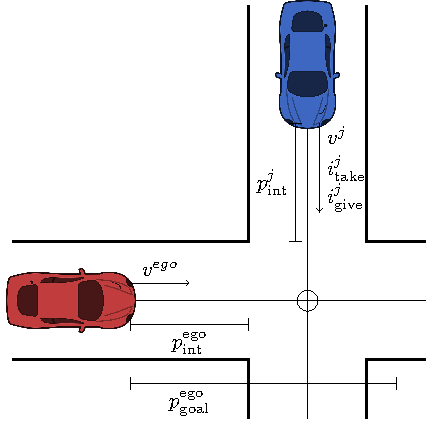
\includegraphics[width=0.6\columnwidth]{figures/figures-observations.pdf}
			\caption{State definitions for the intersection, the red car is the ego vehicle while the blue vehicle represents one of the other vehicles.}
		\label{fig:states}
	\end{figure}
	
	The state of the system,
	\begin{align}
		s = (p^\mathrm{ego}_\mathrm{goal},p^\mathrm{ego}_\mathrm{int}, v^\mathrm{ego}, t_\mathrm{stop}, \{p^{j}_\mathrm{int}, v^j, i^j\}_{j\in 1,\dots,N}),
		\label{eq:state}
	\end{align}
	consists of the ego vehicle state and the states of the surrounding vehicles. The ego vehicle state is described by the distance to the intersection $p^\mathrm{ego}_\mathrm{int}$, the distance to the goal $p^\mathrm{ego}_\mathrm{goal}$ and velocity $v^\mathrm{ego}$. Stop time $t_\mathrm{stop}$ is the time ego is at stand still  $v^\mathrm{ego}=0$, this state tracks the amount of time the ego vehicle has been standing still at the intersection and indicates the time to the terminal states \textit{Safe Stop} or \textit{Deadlock}, that are explained in reward function. The states of the surrounding vehicles, indexed by $j \in 1 \ldots N$, are described by the distance to the intersection $p^{j}_\mathrm{int}$, the velocity $v^j$, and the intention $i^j$. The intentions are represented by a one-hot vector and can be either "give way", which means that the vehicle will stop before the intersection, or "take way", which means that the vehicle will drive through the intersection. These intentions control the behavior of the \gls{idm} model, described in Section~\ref{sec:driver_model}.
	
	%Depending on the different intention, the transition model would be different. One example is when an observed car with a give way intention would slow down, because all cars follow an \gls{idm} it would cause all following cars to slow down behind it. By knowing the intention of the leading car we can more accurately predict the future state of the following car. 
	%However, the intent of other drivers are not something that can be easily measured. Therefore, we propose an observation model to handle the probability of being in either intention states. 
	
	% \jonas{forklara att bilen kan sta still framfor en korstning och endast da okar $t_\mathrm{stop}$, om hastigheter $v=0$ da okar tiden $t$}
	
	% \tommy{-Intention:Other agents follow a \gls{idm}. agents with intention Take way does not have an interaction term when there is no car in front if itself. Agents with intention Give way will include an intention term containing a object with 0 velocity at the center of the intersection. This will cause the agent to slow down to a complete stop right before the intersecting point. Initially each car get random values for each state between an specified interval. }
	
	
	\subsubsection{Observation space, $\Omega$}
	The observations $o$ consist of the ego vehicle state and the physical state of the surrounding vehicles, while the intentions of the surrounding vehicles $i^j$ are not observed. An observation is therefore described by
	\begin{align}
		o = (p^\mathrm{ego}_\mathrm{goal},p^\mathrm{ego}_\mathrm{int}, v^\mathrm{ego}, t_\mathrm{stop}, \{\hat{p}^{j}_\mathrm{int}, \hat{v}^j\}_{j\in1,\dots,N}).
	\end{align}
	
	\subsubsection{Observation model}
	%Ego vehicle have limited information, it knows its own state $s^{\mathrm{ego}}=(p^\mathrm{ego}_\mathrm{goal},p^\mathrm{ego}_\mathrm{int}, v^\mathrm{ego}, t_\mathrm{stop})$ and can only measure the physical states of the other vehicles using sensors, which adds some noise $\sigma$. From the global state $s$, the internal states $(i^j_\mathrm{take},i^j_\mathrm{give})$ are non measurable states. Putting this together the boservable state becomes
	
	% Therefore we use an observation model that gives uf the probability of probability of being in state $s_t$ given the observation $o_t$. In addition, real world sensors also add some noise to the measurements
	% In this paper we model the observed state as the real state plus some noise. A particle filter is used to create a distribution over intention. 
	% \begin{align}
	%     o = (p^\mathrm{ego}_\mathrm{goal},p^\mathrm{ego}_\mathrm{int}, v^\mathrm{ego}, t_\mathrm{stop}, \{p^{j}_\mathrm{int}+\sigma, v^j+\sigma\}_{j\in1,\dots,N}),
	% \end{align}
	
	% where $N$ is the most relevant cars i.e., the cars closest to the intersection. 
	
	The agent observes the ego vehicle states precisely, and a noisy measurement of the positions and speeds of the surrounding vehicles, given by
	%
	\begin{align}
		\label{eq:noise_pos}
		\hat{p}^{j}_\mathrm{int} = p^{j}_\mathrm{int} + \epsilon_\mathrm{p},\\ 
		\hat{v}^j = v^j + \epsilon_\mathrm{v}.
		\label{eq:noise_vel}
	\end{align}
	%
	Here, $\epsilon_\mathrm{p} \sim \mathcal{N}(0, \sigma_p)$ and $\epsilon_\mathrm{v} \sim \mathcal{N}(0, \sigma_v)$.
	% Furthermore, only the $N$ closest vehicles are observed.
	
	
	% \jonas{design val hur manga bilar vi tittar pa}
	
	\subsubsection{Action space, $\mathcal{A}$}
	\label{sec:action}
	The action space $\mathcal{A}$ consists of two high level actions "take way" and "give way". The motion of the ego vehicle is controlled by changing the acceleration using the \gls{idm}, introduced in Section \ref{sec:driver_model}. Depending on the action the \gls{idm} parameters for target vehicle would be different.
	Take way action uses the free term from \eqref{eq:idm_free}, not following any car and just drives though the intersection. 
	The give way action on the other hand uses the interaction term from \eqref{eq:idm_int}, with the variable distance $s$ set to the distance to intersection and the velocity difference $\Delta v_\alpha$ to $0$. 
	This governs the acceleration for the ego vehicle, which in its turn gives us the velocity and position in the next time step. 
	
	\subsubsection{Reward function, $R$}
	\label{sec:reward}
	The reward function is designed to promote a safe and time efficient policy. The main goal of the agent is to reach the goal on the other side of the intersection without colliding with other traffic participants. There are four terminal states: Goal, Safe Stop, Collision and Deadlock. While Goal and collision is self explanatory, Safe stop and Deadlock are reached when the agent chooses to stop at the intersection for $t_\mathrm{stop}$ consecutive seconds.
	To distinguish if a stop was efficient or not, there are two different outcomes. If other vehicles are at stand still and waiting for ego vehicle at the terminal state, the Deadlock reward is received while the safe stop is received if all other cars are in motion while ego is at stand still. The reward function 
	\begin{align*}
	r_t = & \begin{cases}
	8 & \text{reaching the goal,}\\
	0.4 & \text{Safe Stop,}\\
	-10 & \text{Collision},\\
	-0.6 & \text{Deadlock}, \\
	-0.01 & \text{otherwise}
	\label{eq:reward}
	\end{cases} 
	\end{align*}
	is designed to have a big relative difference between the reaching the goal and colliding, with a small incentive for reaching a terminal state faster. While the small reward for safe stop is positive and preferred if the scenario has a lot of cars that does not allow ego to cross. Combined with the negative reward for deadlock, the agent should learn to not stop if the other vehicle is yielding. 
	
	
	\subsubsection{Transition model, $T$}
	The state transition probabilities are implicitly defined by the generative simulation model (Sect.~\ref{sec:simulation_setup}), and not known to the agent.
	
	\subsection{Belief State Estimation using a Particle Filter}
	\label{sec:particle_filter}
	
	To estimate the state of the environment \eqref{eq:state} from noisy observations a particle filter algorithm is proposed that takes advantage of the \gls{idm} and assumptions of observation independence. 
	The role of the particle filter in our method is to estimate the position and velocity of the observed vehicles along with their intention (give way or take way) from noisy measurements of position and velocity. 
	This work does not focus on developing an excellent particle filter but rather to demonstrate how it can be used jointly with a \gls{rl} agent. 
	In particular, we investigate whether it provides any benefits to perform state estimation at training time and whether the decision making agent can be made more efficient by reasoning about a distribution over intentions instead of just a state. 
	
	Previous work has shown that Bayesian filters can be used to infer driver intentions in merging scenarios~\cite{bouton2019}. 
	One challenge in estimating driver intentions is that one might need to consider the joint distribution over the intention of all the drivers interacting in the scenario. 
	In this intersection scenario, a joint estimate of intentions for the four closest drivers is created.
	Each driver is modeled by a position $p^j_\text{int}$, a velocity $v^j$, and an intention $i^j$ which is binary (give way or take way). 
	Let $s^j$ be the three dimensional state of a car. 
	Considering four vehicles at the intersection, the state estimation algorithm must estimate a \num{12} dimensional distribution. A particle filter is used to estimate the state, since the motion of a vehicle can easily be simulated given its intention.% as it does not require knowledge of an explicit transition distribution. 
	
	In order to address the large dimension of the distribution, the fact that the cars are following each other is used to represent the joint transition model as follow:
	\begin{equation}
		\Pr(s_{t+1}^{1:4} \mid s_{t}^{1:4}) = \Pr(s_{t+1}^{1}\mid s_t^1)\prod_{i=2..4}\Pr(s_{t+1}^{i}\mid s_t^i, s_t^{i-1})
		\label{eq:transition}
	\end{equation}
	Without loss of generality it is assumed that the order of vehicles is $1, 2, 3, 4$. Hence the position and speed of vehicle $2$ only depends on the front vehicle $1$ according to the \gls{idm}. In addition, observation of each vehicle are assumed to be independent from each other. 
	Let $o^i_t$ be the observation of vehicle $i$ at time $t$, the joint observation distribution can be expressed as:
	\begin{equation}
		\Pr(o^{1:4}_t \mid s_t^{1:4}) = \prod_{i=1..4}\Pr(o^i_t \mid  s_t^i)
		\label{eq:observation}
	\end{equation}
	Given these two assumptions on the problem structure, the full particle filter procedure can be described. By maintaining a set of $M$ ordered particles for each observed vehicle. A particle representing the joint state can be expressed as follows: $s^{[m]} = (s^{1[m]}, \ldots, s^{4[m]})$, the set of joint particles can be represented by maintaining ordered sets of individual particles for each vehicle. The first particle associated to vehicle 1 will always represent the leading car to the first particle associated to vehicle 2. This assumption allows the implementation to be simpler and more efficient as the statistics for each car can be tracked, noise can be added, or the particle set can be replenish if needed.
	At each time step, the standard particle filter operations of prediction and measurement updates are performed, with a few domain specific improvements.  
	\begin{itemize}
		\item For all particle indices $m$, $s^{\prime[m]}\sim\text{simulate}(s^{[m]})$. Predict the particle one step forward in time using the IDM. The prediction is performed sequentially by updating the leading vehicle first, then its following car, and so on, according to the process described by \eqref{eq:transition}.
		\item Compute observation weights for each particles. A Gaussian sensor model was used for the position and velocity, the weight $w^{[m]}$ of a particle is given by multiplying each of the four vehicle individual weights as described in \eqref{eq:observation}. The individual weights are assumed to follow a Gaussian observation model: 
		\begin{equation}
			w^{j,[m]} \propto \mathcal{N}([p^j_{\text{int}}, v^j]^T ; [\hat{p}^j_\text{int}, \hat{v}^j]^T, \mathrm{diag}[\sigma_p^2, \sigma_v^2])
		\end{equation}
		\item A new set of particles is resampled from the set $\{s^{\prime[m]} | m=1\ldots M\}$ weighted by $w^{[m]}$, if the effective number of particles fall bellow a threshold. 
		% \textit{Stratified resampling} is used in order to maintain a diverse set of particles.
		\item Noise is added to the resampled particles. First by adding some noise to the acceleration in the prediction model. Second, with a slight probability the intention of a particle may switch. This noise models the fact that the transition model is not fully known. 
	\end{itemize}
	At the end of these steps, the set of particles are updated to estimate the current state based on the current observation. The belief of our POMDP agent is represented by the set of resampled particles. 
	
	In order to make the particle filter efficient and avoid known issues such as particle depletion, two improvements were engineered to the process described above. 
	When a vehicle is observed for the first time, a set of $M$ particles are sampled, each individual particle is associated with a joint particle. To respect the intelligent driver model, the position of a new vehicle is sampled uniformly around the first observed position and the position of its leading vehicle, while the velocity is sampled uniformly in the range described in \ref{tab:hyperparameters}. 
	Intentions are initialized as $50\%$ give way and $50\%$ take way. Finally, the state of the individual particles for this new vehicle is appended to the joint particles of the other vehicles that have just been resampled. 
	
	% After the resampling step, we check whether or not the particles associated to a vehicle have converged to a specific intention with \SI{100}{\percent} certainty. If this is the case, we substitute a particle at random and set it to the other attention, the velocity and speed of this new particles are set to match the latest observation of that vehicle. This implementation improvement is analogous to adding noise in the final distribution of particles. 
	
	The particle filter implementation is tailored to the problem of intersection navigation. We take advantage of observation independence, and of the structure of the car following model to efficiently update the set of joint particles. The particles are used to represent the belief state $b$ and the algorithms used train the \gls{rl} agents are described in the next section. 

	\subsection{Belief State Reinforcement Learning}
	\label{sec:belief_state_rl}
	\begin{figure*}[!t]
		\centering
			% \hspace*{-4cm}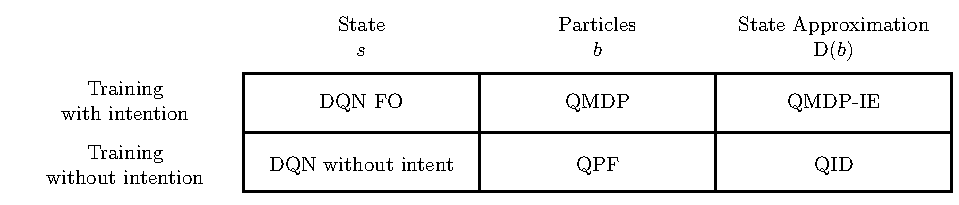
\includegraphics[width=0.85\textwidth]{figures/figures-algorithms.pdf}
			\caption{Table showing the difference between proposed algorithms. The first row are algorithms that have access to the true intention during training, while the algorithms on the second row does not. The columns show the input to the neural network used, where the first column contains the baseline algorithms that use the noisy observation from the sensors either with or without the intention $i^j$. The second column contains algorithms using all $M$ particles as input and the final column uses a estimate of the intention}
		\label{fig:algorithms}
	\end{figure*}
	In this section, the proposed approach to train an \gls{rl} agent in the belief space is described. 
	In classical deep \gls{rl} methods for POMDPs, the learned value function processes a sequence of observations using recurrent neural networks~\cite{HausknechtS15drqn}, or by concatenating a finite history of observations and feeding it to a simple feed forward neural network\cite{Mnih2015}. In this approach, a state estimation algorithm is used instead to compute a belief state based on the sequence of past observation and action. The resulting distribution is then fed to a deep \gls{rl} agent. Instead of processing observations our agent processes belief states. By learning in the belief space our agent is more robust to state uncertainty and, contrary to the QMDP approach, it can compensate for some limitations of the state estimation module. 
	This ability is key to learning intention aware policies for autonomously navigating intersections.
	
	All the proposed algorithms in this paper will follow the same deep Q-learning structure, shown in \ref{alg:training_process}, with the added subtlety that the architecture of the value function, in step $10$, varies in order to process belief states. 
	The loss function in \ref{eq:dqn-loss} takes the form of a mean-squared error with a target corresponding to $r +  \gamma \max_{a\prime}Q(s', a; \theta)$ and a prediction corresponding to $Q(s, a; \theta)$. 
	Depending on the algorithm presented, the prediction will be performed in a different way.
	
	To confirm the hypothesis that the intention state is necessary, two baseline \gls{dqn} algorithms are used. 
	
	\textbf{DQN FO}: This algorithm is trained with full observability and has access to the true intention at training. As mentioned earlier, intention can not directly be measured and therefore this algorithm is just used to show the best policy if the intention approximation is fully accurate. It also assumes perfect observability, without noise, of the other state variables.
	
	\textbf{DQN without intention}: Compared to the previous algorithm, this has access to the same states except the intention. By omitting the intention from the input state that is fed to the neural network, this baseline algorithm can be used to show the limit of a policy that does not have access to the intention.
	
	\textbf{QMDP}: The first approach to process belief state is the QMDP approach described in \ref{eq:qmdp}. 
	The belief state is used at test time but the agent is trained in an environment with full observability in order to estimate $Q_{\text{MDP}}$. The prediction used in the loss function is $Q(s, a)$ and is learned from $(s, a, r, s')$ tuples.
	Although such an approach is very practical, the resulting policy can be sensitive to the performance of the state estimation algorithm used to generate the belief state $b$. 
	To address this issue, we propose to use the true state at training time so that the training procedure matches what the agent will experience at test time. 
	
	\textbf{QPF (Particle Filter)}: With this algorithm, the agent is trained in an environment with partial observability and uses our proposed particle filter algorithm. 
	The input to the agent is a set of $M$ particles. Each particle is fed to the Q-network as a batch for efficient processing which gives us a batch of Q-values.
	The aggregation of the Q-values for each particle is then implemented as part of the computational graph of the deep Q network. 
	The loss function is minimized from $(b, a, r, b')$ experience samples and the Q-learning prediction is given by:
	\begin{equation}
		Q(b, a; \theta) = \frac{1}{M} \sum_{s^{[m]} \in M} Q(s^{[m]}, a; \theta)
	\end{equation}
	This operation is differentiable and allows training $Q(b, a)$ using deep Q-learning. 
	One challenge with this approach is that the number of particles used to represent the belief can be very large in practice and cause the training to be unstable and very slow. It is challenging to update the individual Q-values by back propagating the loss function computed based on an aggregation of the values of many particles.
	
	\textbf{QID (Intention Distribution)}: The agent is also trained in an environment with partial observability and the loss is minimized using $(b, a, r, b')$ samples as well. To simplify the training procedure compared to QPF, the probability distribution of the intention is used to compute the prediction:
	\begin{equation}
		Q(b, a; \theta) = Q(\text{D}(b), a; \theta)
	\end{equation}
	where 
	% $\text{D}(b)$ is the observed kinematic state with the probability distribution from the belief state $b$ for the intention state
	\begin{equation}
		\text{D}(b) = (p^\mathrm{ego}_\mathrm{goal},p^\mathrm{ego}_\mathrm{int}, v^\mathrm{ego}, t_\mathrm{stop}, \{\hat{p}^{j}_\mathrm{int}, \hat{v}^j, \tilde{i}^j\}_{j\in1,\dots,N}),
		\label{eq:IE_b}
	\end{equation}
	and the probability distribution of the intention
	\begin{equation}
		\tilde{i}^j = \sum_{m \in \textbf{particles}} w^{j,[m]} [\tilde{i}_\text{take} , \tilde{i}_\text{give}]^{j,[m]}
	\end{equation}
	is given by the particle filter, where $w^{j,[m]}$ is the weight of the particle $m$ and $[\tilde{i}_\text{take} , \tilde{i}_\text{give}]$ is the one-hot vector specifying the particles intention. 
	This operation does not affect the differentiability of the Q function that is trained using the same procedure as QPF. 
	The advantage of this approach is that at training time, the agent can experience changes in the estimated intention that would match what the state estimator would produce at test time.
	As a consequence, the agent becomes more robust to the error in intention estimation.
	
	\textbf{QMDP-IE (Intention Estimate)}: This last algorithm consists of training an agent on a fully observable MDP just like in the QMDP approach. At test time, instead of averaging the Q-values of each particle, a single intention state is computed from the distribution and use its Q-values to make the decision. Similar to \ref{eq:IE_b}, only the intention is estimated using the particle filter and is represented as a one-hot vector is given by 
	% \todo{if you have a very hogh threshold on the take way intention you onlky have }
	\begin{align}
	\hat{i}^j = & \begin{cases}
	[0 \; 1] & \tilde{i}^j_\text{give} > i_\text{threshold}\\
	[1 \; 0] & \text{Otherwise,}
	\label{eq:IE_i}
	\end{cases} 
	\end{align}
	
	
	Two novel algorithms are proposed QPF and QID which learn belief state value function in a scalable way. 
	By comparing QPF and QID to their respective baseline QMDP and QMDP-IE the results can directly evaluate the benefit of enabling state estimation at training time versus performing it at test time only.
	
	
	
	\section{Experiments}
	\label{sec:experiments}
	In this section the experiment setup, the simulation that generates the different traffic scenarios, the training algorithm and network architecture of the neural network.   
	
	
	\begin{algorithm}[!t]
		\caption{Training process}\label{alg:training_process}
		\begin{algorithmic}[1]
			\State Initialize $\theta$ randomly
			\State $\mathcal{D} \gets \{\}$
			% \State $t \gets 0$
			\For{nr episodes}
				\State $o \gets $ initiate environment
				\State $b \gets $ \Call{InitializeBelief}{$o$}
				\While{episode not finished}
					\If{$e \sim \mathcal{U}(0,1) < \epsilon$}
						\State $a \gets \mathrm{random\ action}$
					\Else
						\State $Q(b, a) \gets $\Call{GetActionValues}{$b, \theta$}
						\State $a \gets \argmax_{a} Q(b,a)$
					\EndIf
					\State $o^\prime, r \gets $ \Call{StepEnvironment}{$a$}
					\State $b^\prime \gets $ \Call{UpdateBelief}{$b$, $o^\prime$, $a$}
					   \State $\mathcal{D} \gets \mathcal{D} \cup \{(b, a, r, b^\prime)\}$
					   \State $M \gets $ sample from $\mathcal{D}$
					   \State update $\theta$ with SGD and loss $J(\theta)$ 
					% \State $t \gets t + 1$
				\EndWhile
			\EndFor
			% \Function{UpdateBelief}{$b_t, \theta$}
			% 
			% \EndFunction
		\end{algorithmic}
	\end{algorithm}
	

	\subsection{Simulator setup}
	\label{sec:simulation_setup}
	
	% \subsubsection{Initial state}
	% The intersections consists of two perpendicular lanes, with one intersecting point. 
	% the ego vehicle starts about $70$ m from the intersection point. With a initial speed of $5$ m/s and a desired speed of $5$m/s. 
	At the start of each episode, up to $N$ number of vehicles are spawned with initial positions $p^j_0$ distributed along the intersecting lane, a starting velocity $v^0$ and a desired velocity $v^j_\mathrm{desired}$. Each vehicle is spawned with a deterministic policy that represents their intention, this can be either take way or give way as described in section \ref{sec:action}. The ego vehicle is spawned last with an initial speed $v^\mathrm{ego}$ and desired speed $v^\mathrm{ego}_\mathrm{desired}$. The starting position of ego is then set based on the time to intersection of one of the other vehicles, assuming constant velocity: 
	
	\begin{equation}
		p^\mathrm{ego}_0 = v^\mathrm{ego} \frac{p^{j\in[1-4]}_0}{v^{j\in[1-4]}_0}
	\end{equation}
	This initialization scheme increases the probability that ego will have a conflict with at least one other car. 
	
	% \subsubsection{Run time}
	The decision time between decisions steps are $\mathrm{d}t_{\text{decision}}$. For every decision step, the simulator updates the objects states four times with a simulation time $\mathrm{d}t_{\text{sampling}}$, checking for terminal states at each update. 
	The simulator keeps track of the true state of all objects. An observation model is used to add noise to each observation, following \ref{eq:noise_pos} and \ref{eq:noise_vel}. The update function updates the true state $s_t$. 
	Every time a vehicle in the perpendicular lane cross the intersection, they are re-spawned at the start of the lane at a random instance with new initial states and intention.
	
	% \subsubsection{terminal state}
	The possible terminal states are the following:
	% \begin{enumerate*}[label=(\roman*)]
	%   \item Goal, ego vehicle reaching the goal.
	%   \item Collision, ego collides with one of the other vehicles.
	%   \item Safe Stop, if ego has been standing still for more than $T_\mathrm{stop}$ seconds.
	%   \item Deadlock, if another vehicle standing still at the intersection yielding for ego and while ego has also been standing still for more than $T_\mathrm{stop}$ seconds. 
	%   \item Finally Timeout, if the total simulation time exceeds $T_{lim}$. 
	% \end{enumerate*}
	Each of these terminal states, except for the simulation timeout, has a corresponding reward, described in Section \ref{sec:reward}. 
	
	\begin{table}[!bt]
		% increase table row spacing, adjust to taste
		\renewcommand{\arraystretch}{1.2}
		\caption{Hyperparameters of Simulator}
		\label{tab:hyperparameters}
		\centering
		\begin{tabular}{l l r}
			\toprule
			%Parameter & Value\\
			sampling time $[s]$, & $\mathrm{d}t_\mathrm{sampling}$ & $0.5$\\
			decision time $[s]$, & $\mathrm{d}t_\mathrm{decision}$ & $2$\\
			initial speed $[m/s]$, & $v^o_0 $ & $2-7$\\
			initial acceleration $[m/s^2]$, & $a^o_0 $ & $0$\\
			desired speed $[m/s]$, & $v_\mathrm{desired}^o$ & $2-7$\\
			time gap $[s]$, & $T_\mathrm{gap}$ & $1.5$\\
			Stop time limit $[s]$, & $T_\mathrm{stop}$ & $10$\\
			Timeout time $[s]$, & $T_\mathrm{lim}$ & $120$\\
			ego spawn speed $[m/s]$, & $v^\mathrm{ego}$ & $5$\\
			ego desired speed $[m/s]$, & $v^\mathrm{ego}_\mathrm{desired}$ & $5$\\
			noise position $[m]$,, & $\sigma_\mathrm{p}$ & $2$\\ 
			noise velocity $[m/s]$,, & $\sigma_\mathrm{v}$ & $1$\\ 
			max observed vehicles, & $N$ & $4$\\ 
	
			\midrule
			IDM max acceleration $[m/s^2]$, & $\alpha^{\mathrm{max}} $ & $0.73$\\
			IDM deceleration $[m/s^2]$, & $\alpha_b $ & $0.5 - 4.0$\\
			IDM acceleration exponent, & $\delta$ & $4$\\
			IDM minimum distance $[m]$, & $s_0$ & $2$\\
			\midrule
			
			number of particles & $n_b$ & 100\\
			acceleration noise $[m/s^2]$ & $\sigma_a$ & 0.1 \\
			intention switch probability & $p_i$ & 5 \\
			intention probability threshold & $i_\text{threshold}$ & 0.8 \\
			\midrule
			
			Batch size & B & $128$ \\
			Learning rate & lr & $0.0001$ \\
			Discount factor & $\gamma$ & $0.95$\\
			Replay memory size & $M_\mathrm{replay}$ & $20{,}000$\\
			Target network update frequency & $N_\mathrm{update}$ & $1{,}000$\\
	
	% 		Initial exploration constant, $\epsilon_\mathrm{start}$  & $1$\\
	% 		Final exploration constant, $\epsilon_\mathrm{end}$ & $0.05$\\
	% 		Final exploration iteration, $N_{\epsilon\mathrm{{\mathrm -}end}}$ & $1{,}000{,}000$\\
	
			\bottomrule
		\end{tabular}
	\end{table}
	

	\subsection{Neural network architecture}
	 The neural network architecture that is used in this study is shown in Fig.~\ref{fig:network}. In a previous study~\cite{Hoel2018}, the use of applying a convolutional operator to the states that describe the surrounding vehicles was introduced. With this structure, the states that describe each surrounding vehicle are passed through the same weights. A more detailed description of the use and advantages of this convolutional operator is given in~\cite{Hoel2018}. The size and stride of the convolutional layer is set to $(4, 1)$, where four equals the number of states that describe each vehicle and one means that the different particles are handled individually. The convolutional layer uses \num{32} filters with a $\tanh$ activation function. To speed up the learning, the index $j$ are ordered by distance $p^j_\mathrm{int}$ starting from the vehicle closest to the intersection and a default state are used for cars that does not exist. 
	
	The states that describe the ego vehicle are passed through a fully connected layer of size $32$, before being concatenated with the output of the convolutional layer. The output of the concatenated layer is then passed through two fully connected layers of size $32$ and finally a fully connected layer of size two gives the $Q$-values for each particle. These values are then merged according to one of the algorithms in Sect.~\ref{sec:belief_state_rl} to form a combined estimate of the $Q$-values. The belief dimension of the neural network represents the number of particles $n_b$ that are passed through the network. This number varies depending on which algorithm that is used, see Sect.~\ref{sec:belief_state_rl}.
	
	
	
	\begin{figure}[!t]
		\centering
			% 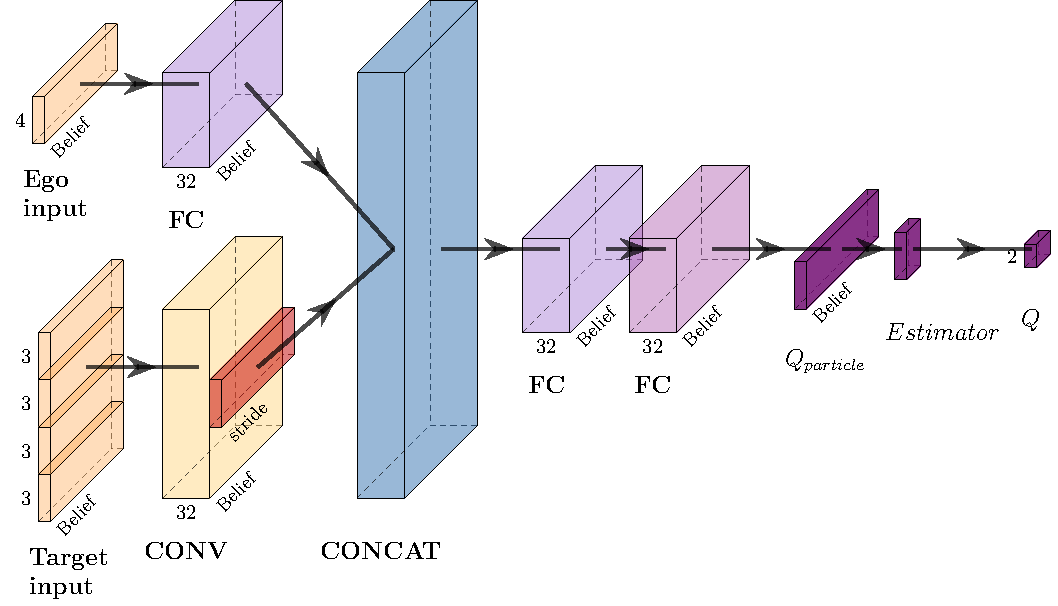
\includegraphics[width=0.9\columnwidth]{figures/belief.pdf}
			\caption{Network architecture, where Ego input represents the input features for the ego vehicle, $p^\mathrm{ego}_\mathrm{goal},p^\mathrm{ego}_\mathrm{int}, v^\mathrm{ego}, t_\mathrm{stop}$, and Target input $\{p^{j}_\mathrm{int}, v^j, i^j\}_{j\in 1,\dots,N}$ for the the target vehicle $j$. The layers consists of one convolution (Conv) and a total of three Fully connected (FC), where the depth of the layers represents the belief size.}
		\label{fig:network}
	\end{figure}
	
	\subsection{Training Procedure}
	Each network was trained for \num{200000} episodes. The loss function of Double DQN is applied, which subtly modifies the maximization operation of \ref{eq:dqn-loss} to $\gamma Q(s',\argmax_{a'} Q(s',a';\theta_i);\theta_i^-)$~\cite{Hasselt2016}. 
	Stochastic Gradient Decent is used to update the weights~\cite{Kingma2014}. The hyper parameters of the training process are shown in Table~\ref{tab:hyperparameters}, and the values were selected by an informal search, due to the computational complexity. 
	
	If the current policy of the agent does not reach a terminal state before the simulation timeout time $T_\mathrm{lim}$, an episode in the real world could continue forever. Therefore, when the simulation reaches the timeout state the last experience of such an episode is not added to the replay memory. This trick prevents the agent to learn that an episode can end due to a timeout, since the terminating state is not part of the MDP~\cite{Hoel2018}.
	
	\section{Results / Results and discussion}
	\label{sec:results}
	In this section the evaluation metrics and results are presented. The results are presented in Table \ref{tab:results_summary} is a summary of the most complex scenario with four other target cars in the intersection. 
	
	Each agent is evaluated on \num{1000} episodes for different numbers of cars separately. The random seeds are set based on the episode number, which gives the same test scenarios between different agents.
	The metrics of interests are the average time it takes for the agent to either reach success state and how often each terminal state is reached. A success state refers to either reaching the goal or a safe stop, where both are considered good outcomes. The priority is first to find an agent that with zero collisions and zero deadlocks, then look at the time it takes to reach the goal. 
	% Figure \ref{fig:number_cars}, shows the performance metrics for the baseline algorithm DQN without intention for scenarios with different number of cars. From this figure, it can be observed that the problem becomes more difficult to solve for the highest number of crossing vehicles, hence we use the scenario with four crossing cars to compare the performance between the algorithms and the results are presented in Table \ref{tab:results_summary}.
	
	\begin{figure}[!t]
		\centering
			% \includegraphics[width=0.99\columnwidth]{figures/results Scenarios 1-4 Target Cars.png}
			\caption{Performance results for DQN without intention algorithm, showing the increasing difficulty for scenarios with different number of cars in the environment.}
		\label{fig:number_cars}
	\end{figure}
	
	
	\begin{table}
	\caption{Result summary for N=4 cars}
	\label{tab:results_summary}
	\begin{tabularx}{\columnwidth}{@{}l*{10}{c}c@{}}
	\toprule
	Experiments     & Goal Reached & Safe Stop & Collision & Deadlock & Success Time & Training Time\\ 
	\midrule
	DQN FO & $94.20$ & $5.60$ & $\textbf{0.00}$ & $0.20$ & $16.93$ & $1d7h$ \\ 
	DQN w/o intent & $94.10$ & $2.80$ & $1.10$ & $2.00$ & $18.29$ & $1d7h$ \\ 
	QMDP & $93.70$ & $5.60$ & $\textbf{0.10}$ & $0.60$ & $19.95$ & $1d7h$ \\ 
	QMDP-IE & $94.70$ & $4.80$ & $\textbf{0.00}$ & $0.50$ & $17.60$ & $1d7h$ \\  
	QPF & $84.70$ & $8.90$ & $3.60$ & $2.80$ & $20.16$ & $2d17h$ \\ 
	QID & $\textbf{97.00}$ & $0.90$ & $2.00$ & $0.10$ & $\textbf{16.90}$ & $2d10h$ \\ 
	\bottomrule
	\end{tabularx}
	\end{table}
	
	\begin{figure}[!t]
		\centering
			% \includegraphics[width=0.99\columnwidth]{figures/results Evaluation Results.png}
			\caption{Visual representation of the results from Table \ref{tab:results_summary}. Starting from the two baseline algorithms DQN with and without access to the intention state. Followed by the algorithms that has access to the intention state at training, QMDP and QMDP-IE. Finally the two algorithms that does not have access to the intention, QPF and QID.}
		\label{fig:results_summary}
	\end{figure}
	

	\subsection{Baseline DQN results}
	The agent trained with full observability, DQN FO, shows how well an agent could perform if it had access to the true intention of other drivers. Table \ref{tab:results_summary} shows that the policy has \SI{0}{\percent} collisions, \SI{5.6}{\percent} safe stops, \SI{.2}{\percent}, deadlocks, \SI{94.2}{\percent} goals reached and an average success time of \SI{16.93}{\second}. 
	This confirm our hypothesis that having an intention state is necessary to find the best policy. DQN with intention was both faster to reach the goal and could do it with zero collisions.
	While DQN without intention ended up in collisions \SI{1.1}{\percent} of the episodes, followed by \SI{2.0}{\percent} in deadlock, \SI{2.8}{\percent} in safe stop, \SI{94.1}{\percent}  in goal reached, with a slower average time of \SI{18.29}{\second}.  All agents are trained with a variable number of other vehicles and \ref{fig:number_cars} shows that in scenarios with only one other vehicle, the agent trained using DQN without intention found a policy that could avoid collisions. Increasing the number of other vehicles makes the problem harder to solve, which results in an increasing number of collisions and a longer success time. 
	% This confirms the hypothesis that the intention state is important and will improve the policy by reaching the goal faster and end up in collision and deadlock states less often.  
	
	% and an agent trained without the intention as input are shown in figure \ref{fig:baseline_results}. The time it takes for the agent to reach the goal is longer and the number of times the agent ends up in a collision state is higher. This motivates that the intention is necessary to solve the MDP strengthening the hypothesis that this is a \gls{pomdp}. 

	
	
	\subsection{QMDP and QMDP-IE results}
	QMDP and QMDP-IE are both approximation algorithms that use the network trained on DQN FO and they both achieve zero collisions, have similar safe stop of around \SI{5.6}{\percent} and \SI{0.6}{\percent} deadlocks. Compared to DQN without intention, QMDP is more conservative with a slower success time of \SI{19.95}{\second}, while the QMDP-IE is faster with \SI{16.90}{\second}. \ref{fig:intent_threshold} shows the performance for different threshold values of $i_\text{threshold}$. With $i_\text{threshold}=0.5$ being equivalent to just taking the most likely estimation of the intention, it also has the most aggressive behaviour with around \SI{1}{\percent} collisions, \SI{0.8}{\percent} deadlocks but reaches the goal in \SI{17.3}{\second}. While an agent with $i_\text{threshold}=0.8$ achieve zero collisions, \SI{0.5}{\percent} deadlocks and manages to reach the goal in \SI{17.6}{\second}. As the threshold value increases so does the safe stop rate and the time it takes to reach the goal. 
	
	\begin{figure}[!t]
		\centering
			% \includegraphics[width=0.99\columnwidth]{figures/results Intention threshold.png}
			\caption{QMDP-IE performance results for different $i_\text{threshold}$ values along the x-axis.}
		\label{fig:intent_threshold}
	\end{figure}

	The proposed particle filter does a decent job of estimating the probability distribution of the intention, but it relies on having a prediction model and the accuracy was very correlated with the noise of the probability distribution. 
	This could be improved by increasing the number of particles. However, that would also increase the required computational power and the hardware in AVs today does not necessarily have sufficient memory capacity. 
	
	\subsection{QPF and QID results}
	Finally, the algorithms that do not have access to the intention during training, have the lowest number of goal reached. QPF has the lowest goal rate at \SI{84.7}{\percent}, the highest collision rate at \SI{3.6}{\percent} and the slowest with an average success time of \SI{20.16}{\second}, followed by a \SI{8.9}{\percent} safe stop and \SI{2.8}{\percent} deadlocks. An interesting observation is that QID learned the most aggressive policy, having the lowest success time \SI{15.71}{\second}, which is lower than DQN baseline algorithm. But the consequence is that it has a slightly higher collision rate at \SI{1.9}{\percent}. Finally, it took almost two and a half days to train QPF and QID which is almost twice as much time it took to train the fully observable network. 
	
	

	
	\subsection{discussion}
	% \todo{PF are super tricky to get to work and it is even harder to use them as input.}
	\label{sec:discussion}

	\textit{Is it better to train on the full distribution of the belief or use an estimation of the intention?} When comparing QPF and QID to their baselines, it is observed that both algorithms that were trained on the ground truth outperform the algorithms that were trained using the belief state or even just an estimate of the belief distribution. Both QMDP and QMDP-IE could maintain zero collisions just like DQN FO, while QMDP-IE had a slightly faster policy. 
	
	\ref{fig:intent_threshold} shows that the aggressiveness of the policy from QMDP-IE is correlated with $i_\text{threshold}$ and by choosing a relatively high value at $0.8$ the policy could achieve zero collisions and in this case could compensate for the loosely optimized particle filter. The ability to adjust the aggressiveness of the policy by changing $i_\text{threshold}$ is also a strength of QMDP-IE compared to our previous black box methods that use \gls{lstm} to estimate the hidden state \cite{Tram2018}. For QMDP and QMDP-IE, it is not unreasonable to assume that the true intention of other drivers is accessible during training. These intentions can be labeled after the fact, by looking at if the driver ended up crossing the intersection or stopping before it. 
	
	We used a particle filter to create the belief state and filter the noisy observations, hoping the flexibility of the neural network would be able to compensate for some of the inaccuracy of the belief in the same way it can approximate the noise. The higher collision rate for the QPF compared to QMDP shows that training on the full set of beliefs have a harder time finding a good policy, while the time to goal was also very similar. 
	% The results showed that the algorithms that trained on the information from the particles had a harder time to converge. The network trained with the QPF algorithm often got stuck in some local minima and ended up in either always take way or always give way policy. 
	% The results showed around \SI{2.4}{\second} difference between the QMDP and QMDP-IE for the ego vehicle. Although \SI{2.4}{\second} does not seem to be that much for average time, but could accumulate to be a lot when there are several ego agents in the same lane trying to cross this intersection. 
	
	The terminal state referred to as collision in this paper may sound drastic, but could also be interpreted as intervention by a collision avoidance system. Because the goal of the agent is mainly to  

	\section{Conclusion}
	\label{sec:conclusion}
	In this paper, we compared five algorithms that find an policy to drive through an intersection with crossing traffic participants that has a hidden intention state. We confirmed the hypothesis that knowing the intention state for crossing drives increases the performance of the agent by comparing a DQN agent with the true intention as an input state and an agent trained without the intention state. 
	Two algorithms, QMDP and QMDP-IE, use a network trained with access to the true intention state of the other vehicles but was evaluated with an estimate of their intention. Both algorithms could find a policy with zero collisions, while QMDP-IE lead to the most efficient policy, Whereas QPF and QID, that were trained without access to the true intention state could not achieve a policy without collisions. 
	However, the QID agent had the fastest average time to reach the goal. The results for the QPF agent, showed that training on the entire belief state as input had the worst performance out of all the algorithms and motivates the need for a network structure can learn the hidden state better like Deep Variational Reinforcement Learning proposed by Igl et al.~\cite{Igl2018}. 
	